\documentclass[a4paper]{exam}
\usepackage{graphicx}
\usepackage{cmbright}
\usepackage{caption}
\usepackage{subcaption}
\usepackage{multirow}
\usepackage{siunitx}
\usepackage{svg}
\usepackage{minted}

\firstpageheader{EE5907}{CA2}{\today}
\runningheader{EE5907}{CA2 (Continued)}{\today}
\footer{}{\thepage}{}

\graphicspath{ {figures/} }

\newcommand\percentage[2][round-precision = 2]{% default precision: 2
    \qty[round-mode = places,
        scientific-notation = fixed, fixed-exponent = 0,
        output-decimal-marker={.}, #1]{#2e2}{\percent}%
}


\begin{document}
PCA and LDA were implemented using NumPy \cite{2020NumPy-Array}.
Other algorithms were functions provided directly by Python packages,
namely GMM from scikit-learn \cite{scikit-learn}, SVM from LIBSVM \cite{CC01a} and CNN from Tensorflow \cite{Abadi_TensorFlow_Large-scale_machine_2015}.

For both LDA and CNN, which do not reference PCA like GMM and SVM, the full training dataset was used.
In particular, density of visualized points is too low for LDA with only $500$ points.

As the PIE images are labelled 1 to 68, I labelled my selfies as 69.
For the scatter pots, colors are repeated as there is no convenient way to obtain a color directly from a number in Matplotlib,
and the maximum number of colors in the colormaps seems to be $20$. Selfies are distinguished with a red star.

The $25$ subjects chosen are 67, 30, 59, 44, 66, 53, 34, 54, 19, 29, 17, 45, 52, 16, 46,  4, 15,
11, 32, 61, 21,  2, 27, 35 and 23.

\begin{questions}
    \question PCA based data distribution visualizations

    Let the data matrix $\mathbf{X}$ be of $n \times p$ size.\\
    First, perform SVD:
    \begin{equation}
        \mathbf{X}=\mathbf{USV^T}
    \end{equation}
    The columns of $\mathbf{XV}=\mathbf{USV^TV}=\mathbf{US}$ are the principal components and the columns of $\mathbf{V}$ are the eigenfaces.\\
    For the principal components, only calculation for the highest dimension is necessary. For reduction to
    dimension $k$, the first $k$ principal components can be obtained from the first $k$ columns of
    $\mathbf{U}$ and the diagonal matrix formed by the first $k$ values along the diagonal of $\mathbf{S}$.

    \begin{figure}[h]
        \centering
        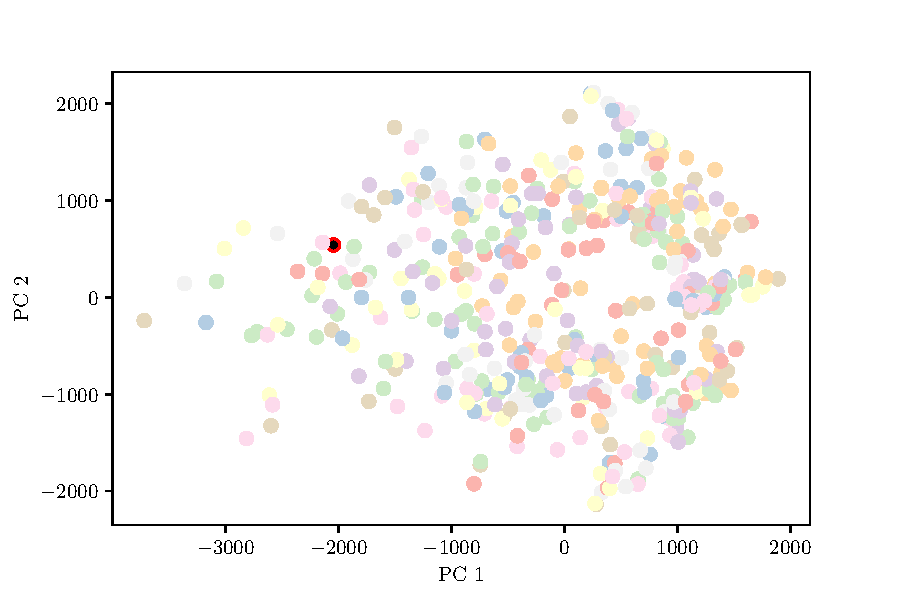
\includegraphics[width=0.75\textwidth]{pca_2d}
        \caption{PCA projected data vector in 2D.}
        \label{fig:pca_2d}
    \end{figure}

    \begin{figure}[ht]
        \centering
        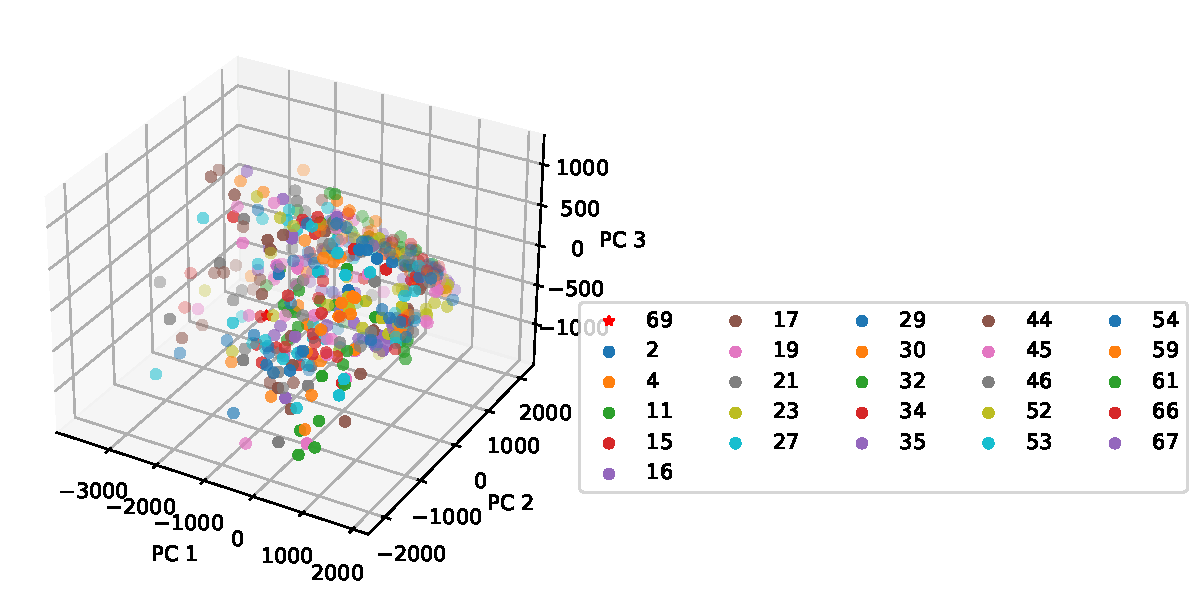
\includegraphics[width=0.75\textwidth]{pca_3d}
        \caption{PCA projected data vector in 3D.}
        \label{fig:pca_3d}
    \end{figure}

    \begin{figure}[ht]
        \centering
        \begin{subfigure}[b]{0.3\textwidth}
            \centering
            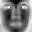
\includegraphics[width=\textwidth]{eigenface0}
            \caption{eigenface 0}
            \label{fig:eigenface0}
        \end{subfigure}
        \hfill
        \begin{subfigure}[b]{0.3\textwidth}
            \centering
            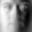
\includegraphics[width=\textwidth]{eigenface1}
            \caption{eigenface 1}
            \label{fig:eigenface1}
        \end{subfigure}
        \hfill
        \begin{subfigure}[b]{0.3\textwidth}
            \centering
            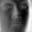
\includegraphics[width=\textwidth]{eigenface2}
            \caption{eigenface 2}
            \label{fig:eigenface2}
        \end{subfigure}
        \caption{Corresponding 3 eigenfaces used for PCA dimensionality reduction.}
        \label{fig:eigenface}
    \end{figure}

    \clearpage\question PCA plus nearest neighbor classification results

    For classification with PCA, obtain $\mathbf{XV}$, projection of the faces in the test data matrix $\mathbf{X}$ on the
    eigenface space. Each column of $\mathbf{V}$ and therefore each column of $\mathbf{XV}$ corresponds to a principal component.\\

    It is expected that classfication of selfies is unsuccessful. There are only three selfies in the test
    set and random sampling of 500 images for training included only one selfie which is an outlier in 3D as can be seen from the scatter plots.
    Moreover, my setup and lighting condition differs from those of the images in the PIE data set.
    illumination is a challenge for many computer vision problems.

    \begin{table}
        \centering
        \begin{tabular}{ |c|c|c|c| }
            \hline
            Test Images                & Dimensionality & Accuracy                           \\
            \hline
            \multirow{3}{4em}{CMU PIE} & $40$           & \percentage{0.4894117647058824e2} \\
                                       & $80$           & \percentage{0.5231372549019608e2}  \\
                                       & $200$          & \percentage{0.5529411764705883e2}   \\
            \hline
            \multirow{3}{4em}{Selfies} & $40$           & \qty{0}{\percent}                  \\
                                       & $80$           & \qty{0}{\percent}                  \\
                                       & $200$          & \qty{0}{\percent}                  \\
            \hline
        \end{tabular}
        \caption{\label{tab:pca}KNN classification accuracy for dimensionalities $40$, $80$ and $200$ after PCA with $500$ samples, for PIE images and selfies.}
    \end{table}

    \clearpage\question LDA based data distribution visualization

    The Fisher-LDA optimization problem is
    $$
        \max_w \frac{w^TS_bw}{w^TS_ww}
    $$
    wehre $S_b$ and $S_w$ are between- and within-class scatter matrices
    $$
        S_b=\sum_{i=1}^N n_i(\mu_i-\mu)(\mu_i-\mu)^T\ \text{and}\ S_w=\sum_{i=1}^N\sum_{x\in \mathcal{C}_i}(x-\mu_i)(x-\mu_i)^T
    $$
    The solutions are the eigenvectors of $S_w^{-1}S_b$, in descending order of the corresponding eigenvalues.
    Perform projection as with PCA.

    Unlike PCA, which does not consider the class labels, projected points belonging to the same class are grouped together.

    \begin{figure}[h]
        \centering
        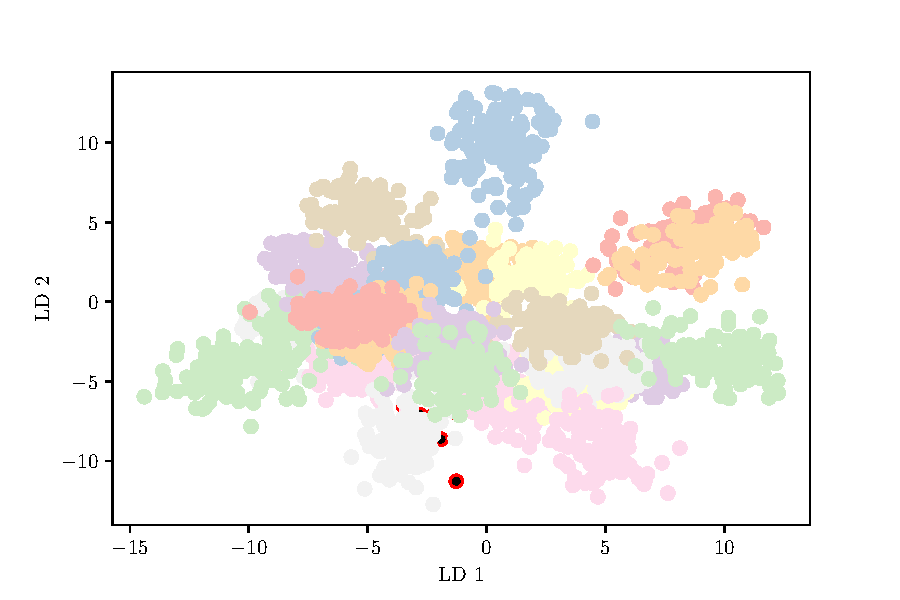
\includegraphics[width=0.75\textwidth]{lda_2d}
        \caption{LDA projected data vector in 2D.}
        \label{fig:lda_2d}
    \end{figure}

    \begin{figure}[ht]
        \centering
        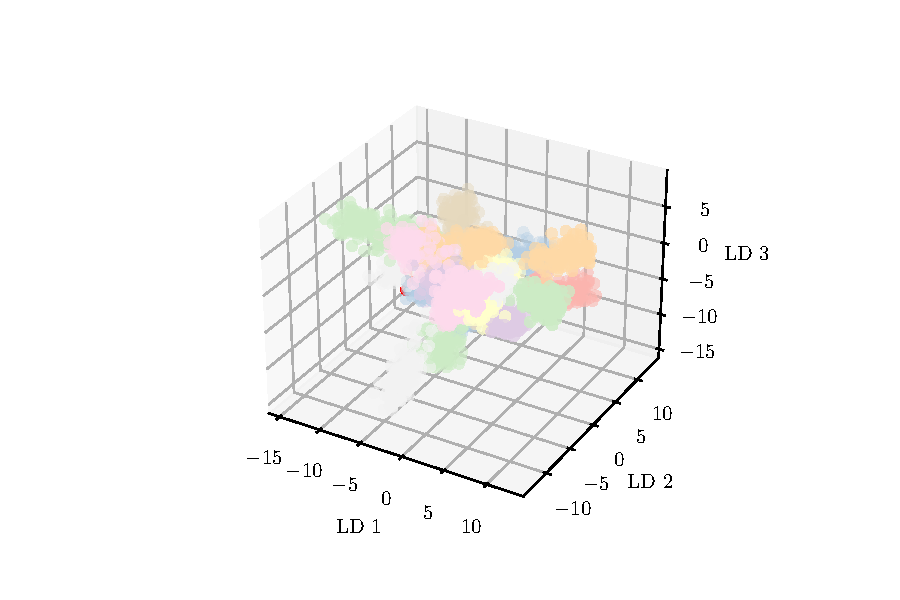
\includegraphics[width=0.75\textwidth]{lda_3d}
        \caption{LDA projected data vector in 3D.}
        \label{fig:lda_3d}
    \end{figure}

    \clearpage\question LDA plus nearest neighbor classification results

    For a fair comparison of PCA and LDA, PCA is rerun with the full training set.

    Clearly, LDA is able to achieve the same classification accuracy with significantly fewer dimensions.
    Exceeding PCA at $40$ dimensions using only $9$ dimensions.

    In general, PCA finds the directions of maximal variance while LDA finds a feature subspace that maximizes class separability.
    While PCA is suitable for feature extraction, LDA is better for classification, as it considers separately the within class and between class variances, minimizing the former while maximizing the latter.

    It is worth noting that $LDA$ succeeds in identifying one out of three selfies with $9$ dimensions.
    Given the difference between my selfies and the PIE images taken under more standardized conditions,
    LDA's consideration of within class variance allows it to be more successful at classiying my selfies,
    which would be outliers among the PIE images.

    \begin{table}[h]
        \centering
        \begin{tabular}{ |c|c|c|c| }
            \hline
            Test Images                & Dimensionality & Accuracy                          \\
            \hline
            \multirow{3}{4em}{CMU PIE} & $2$            & \percentage{0.4768627450980392e2} \\
                                       & $3$            & \percentage{0.6815686274509803e2} \\
                                       & $9$            & \percentage{0.9419607843137255e2} \\
            \hline
            \multirow{3}{4em}{Selfies} & $2$            & \qty{0}{\percent}                 \\
                                       & $3$            & \qty{0}{\percent}                 \\
                                       & $9$            & \percentage{0.3333333333333333}   \\
            \hline
        \end{tabular}
        \caption{\label{tab:lda}KNN classification accuracy for dimensionalities $2$, $3$ and $9$ after LDA, for PIE images and selfies.}
    \end{table}

    \begin{table}[h]
        \centering
        \begin{tabular}{ |c|c|c|c| }
            \hline
            Test Images                & Dimensionality & Accuracy                          \\
            \hline
            \multirow{3}{4em}{CMU PIE} & $40$           & \percentage{0.9388235294117647e2} \\
                                       & $80$           & \percentage{0.96e2}               \\
                                       & $200$          & \percentage{0.9725490196078431e2} \\
            \hline
            \multirow{3}{4em}{Selfies} & $40$           & \qty{0}{\percent}                 \\
                                       & $80$           & \qty{0}{\percent}                 \\
                                       & $200$          & \qty{0}{\percent}                 \\
            \hline
        \end{tabular}
        \caption{\label{tab:full-pca}KNN classification accuracy for dimensionalities $40$, $80$ and $200$ after PCA, for PIE images and selfies.}
    \end{table}

    \clearpage\question GMM for clustering

    For GMM, the clustering result appears to be heavily influenced by shadows or dark regions in general.
    Each cluster occupies a row above their associated scatter plot, with every 15th face shown, up to a limit of 10.
    Regardless of how or whether the input was processed, there is always one row that is of relatively uniform gray level (within each image), one row with dark region on the left, and one row with dark region on the right.
    The algorithm does not appear to be grouping people with similar facial features together, with a European and an Asian appearing together in every cluster.

    Consider the fact that we set the number of components to be $3$. There are a lot of variations in facial features, but patches of black, regions of relatively darkness are much more uniform.
    Therefore, the algorithm is working exactly as intended and grouping the most similar images together, those with the same illumination.

    For clustering by facial features, we would need to set the number of components to be the number of distinct faces in the dataset. With $3$ components, we are doing clustering by illumination.

    Clustering by illumination also means that PCA, which finds components reflecting the largest sources of variance works extremely well for reducing the number of dimensions.
    In this case, illumination is the largest source of variation.

    \begin{figure}[h]
        \centering
        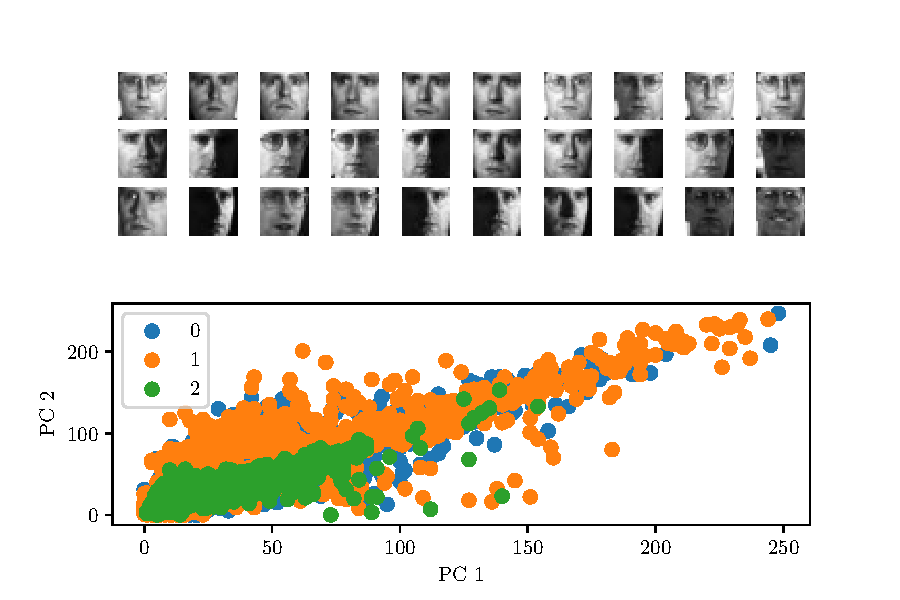
\includegraphics[width=0.75\textwidth]{gmm_1024}
        \caption{GMM clustering for raw face images (vectorized).}
        \label{fig:gmm_1024}
    \end{figure}

    \begin{figure}[h]
        \centering
        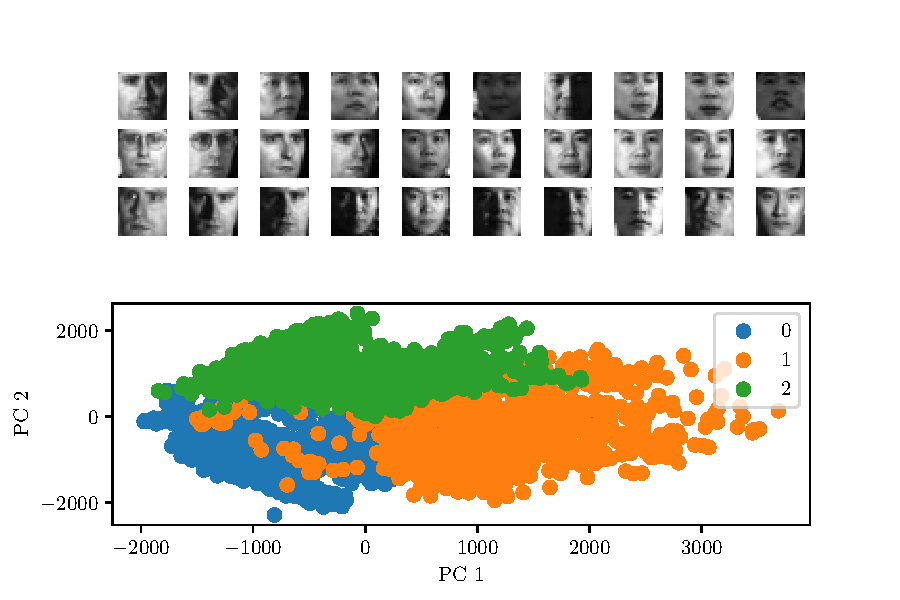
\includegraphics[width=0.75\textwidth]{gmm_200}
        \caption{GMM clustering for face vectors after PCA pre-processing (with dimensionality of 200).}
        \label{fig:gmm_200}
    \end{figure}

    \begin{figure}[h]
        \centering
        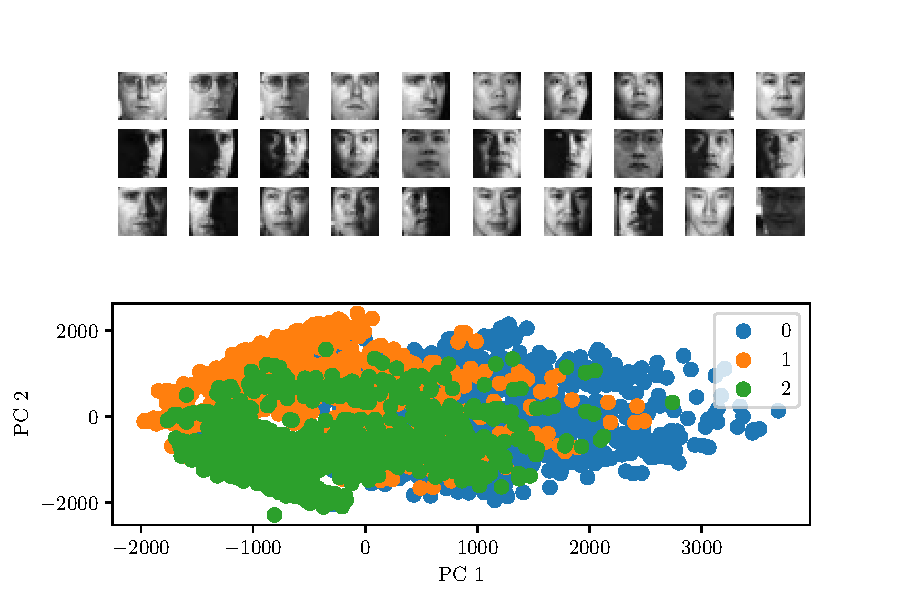
\includegraphics[width=0.75\textwidth]{gmm_80}
        \caption{GMM clustering for face vectors after PCA pre-processing (with dimensionality of 80).}
        \label{fig:gmm_80}
    \end{figure}
    \clearpage\question SVM classification results with different parameter values

    From Tab.~\ref{tab:svm}, we can see that SVM classification achieves much higher accuracy than that of KNN in Tab.~\ref{tab:pca}.
    More principle components improves the classification accuracy, with $200$ principle components, the classfication accuracy is the same as using raw images.

    However, the parameter $C$ appears to have no impact on the classfication accuracy.
    There is an explanation online for this \cite{238209}.
    Of the two criteria, the use of a linear SVM is stated in the instructions for this assignment.

    According to Rasmussen \& Williams \cite{10.5555/1162254}, ``In a feature space of dimension $N$, if $N>n$ then there will always be a separating hyperplane.
    However this hyperplane may not give rise to good generalization performance, especially if some of the labels are incorrect.''

    For $PCA$, $500$ data points were sampled, less than $1024$. The data is linearly separable, meeting the other criterion.

    Therefore, ``if $C$ values change within a reasonable range, the optimal hyperplane will just randomly shift by a small amount within the margin (the gap formed by the support vectors).
    Intuitively, suppose the margin on training data is small, and/or there is no test data points within the margin too, the shifting of the optimal hyperplane within the margin will not affect classification error of the test set.''

    \begin{table}[hb]
        \centering
        \begin{tabular}{ |c|c|c|c| }
            \hline
            Test Images                  & C    & Accuracy                \\
            \hline
            \multirow{3}{4em}{Raw}       & 0.01 & \qty{98.4351}{\percent} \\
                                         & 0.1  & \qty{98.4351}{\percent} \\
                                         & 1    & \qty{98.4351}{\percent} \\
            \hline
            \multirow{3}{4em}{PCA (200)} & 0.01 & \qty{98.4351}{\percent} \\
                                         & 0.1  & \qty{98.4351}{\percent} \\
                                         & 1    & \qty{98.4351}{\percent} \\
            \hline
            \multirow{3}{4em}{PCA (80)}  & 0.01 & \qty{97.9656}{\percent} \\
                                         & 0.1  & \qty{97.9656}{\percent} \\
                                         & 1    & \qty{97.9656}{\percent} \\
            \hline
        \end{tabular}
        \caption{\label{tab:svm}SVM classification accuracy for dimensionalities $40$, $80$ and $200$ after PCA.}
    \end{table}

    \clearpage\question CNN classification results with different network architectures

    For CNN, the accuracy ranges from \percentage{0.95e2}to \percentage{0.97} with shuffling of the order of images.

    Following the updated instructions received via email, my model includes two convolutional layers and two fully connected layers.
    The updated number of nodes is ``20-50-500-26''.
    There is an additional scaling layer at the start to scale the range of each pixel from the range \numrange[range-phrase = --]{0}{255} to \numrange[range-phrase = --]{0}{1}.
    Although often recommended, scaling does not seem to improve the classfication accuracy of this model.

    For previous parts of this assignment, labels were taken directly from the folder names in the provided PIE dataset.
    However, for CNN, one hot encoding is necessary because there is no natural ordinal relationship for the order of PIE subjects.
    For classification of two or more labels using one-hot encoded representation, categorical crossentropy is the option in Keras.
    The final layer uses a softmax function to convert logits to probabilities. Otherwise, ReLU is used to introduce nonlinearity.

    The latest optimizer offered by Keras, the AMSGrad variant of ADAM was used for best performance.
    As ADAM is an adaptive algorithm, no tuning of the learning rate was necessary or offered any improvement to classfication accuracy.

    \begin{listing}[!ht]
        \begin{minted}{text}
        Model: "sequential"
        _________________________________________________________________
         Layer (type)                Output Shape              Param #   
        =================================================================
         rescaling (Rescaling)       (None, 32, 32, 1)         0         
                                                                         
         conv2d (Conv2D)             (None, 28, 28, 20)        520       
                                                                         
         max_pooling2d (MaxPooling2D  (None, 14, 14, 20)       0         
         )                                                               
                                                                         
         conv2d_1 (Conv2D)           (None, 10, 10, 50)        25050     
                                                                         
         max_pooling2d_1 (MaxPooling  (None, 5, 5, 50)         0         
         2D)                                                             
                                                                         
         flatten (Flatten)           (None, 1250)              0         
                                                                         
         dense (Dense)               (None, 500)               625500    
                                                                         
         dense_1 (Dense)             (None, 26)                13026     
                                                                         
        =================================================================
        Total params: 664,096
        Trainable params: 664,096
        Non-trainable params: 0
        _________________________________________________________________
        \end{minted}
        \caption{Summary of CNN.}
        \label{listing:1}
    \end{listing}


    For simplicity, I arbitrarily set the number epochs to $100$ with batch size of $128$.

    It takes about $55$ epochs to reach \qty{100}{\percent} accuracy on the training set and for the training loss to fall from an initial value of about $3.25$ to $0$.

    \begin{figure}[hb]
        \centering
        \includesvg[width=0.75\textwidth]{epoch_accuracy}
        \caption{Epoch accuracy.}
        \label{fig:epoch_accuracy}
    \end{figure}

    \begin{figure}[htb]
        \centering
        \includesvg[width=0.75\textwidth]{epoch_loss}
        \caption{Epoch loss.}
        \label{fig:epoch_loss}
    \end{figure}
\end{questions}
\clearpage
\bibliographystyle{IEEEtran}
\bibliography{refs}
\end{document}
